\section{Implémentation}
\subsection{Prototype initial en Matlab}

Le prototype initial s'est fait au moyen de Matlab et des solveurs \texttt{quadprog} pour la génération de trajectoire et \texttt{fmincon} pour l'optimisation des temps de trajectoire. Pour commencer nous avons reproduit les résultats de Mellinger en faisait une trajectoire simple à travers les points $(0,0)$, $(1,0)$, $(1,2)$ et $(0,2)$ avec une allocation de temps égale à chaque segment de trajectoire et aucune contrainte sur les derivées, outre celles de continuité.

\begin{figure}[h]
\centering
\begin{subfigure}{.4\textwidth}
  \centering
  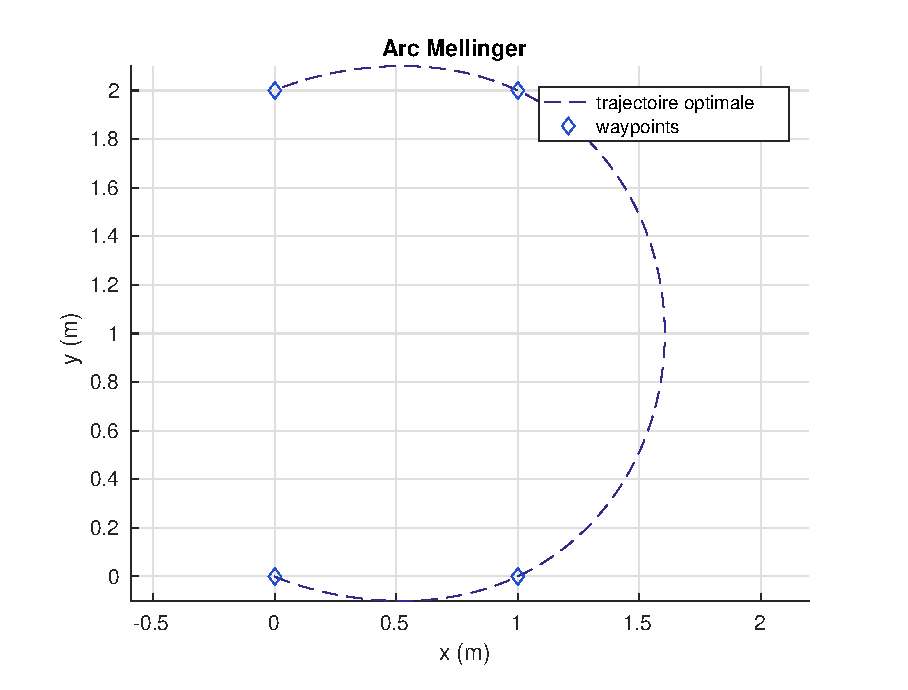
\includegraphics[width=\textwidth]{fig/arc_mellinger}
  \caption{Notre résultat}
\end{subfigure}%
\begin{subfigure}{.4\textwidth}
  \centering
  \includegraphics[width=0.6\textwidth]{fig/arc_mellinger_orig.png}
  \caption{Résultat de Mellinger \cite{Mellinger2011}}
  \label{fig:sub2}
\end{subfigure}
\caption{Comparaison de résultats}
\label{fig:comparaison}
\end{figure}

Nous voyons dans la figure (\ref{fig:comparaison}) que nous obtenons presque les mêmes résultats que dans \cite{Mellinger2011}. La différence entre les deux solutions pourrait  être reliée aux paramètres d'optimisation de \texttt{quadprog} ou les paramètres de tolérance sur la solution. D'ailleurs, Mellinger ne spécifie pas quel solveur il a utilisé pour résoudre le problème QP.


\begin{figure}[htp]
\centering
\begin{subfigure}{.45\textwidth}
  \centering
  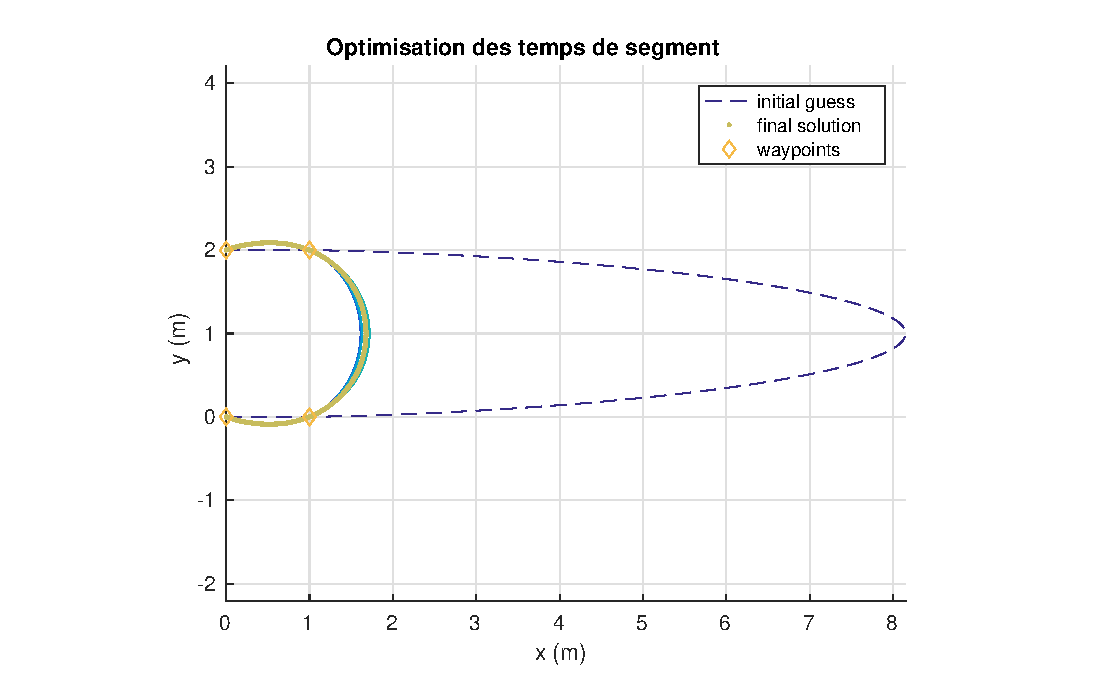
\includegraphics[width=1.2\textwidth]{fig/arc_time_opt}
  \caption{Résultat des itérations, l'allocation de temps initiale donnait beaucoup trop de temps au segment du milieu.}
\end{subfigure}%
\begin{subfigure}{.45\textwidth}
  \centering
  \includegraphics[width=\textwidth]{fig/cost}
  \caption{Valeur de la fonction de coût à chaque itération}
  \label{fig:sub2}
\end{subfigure}
\caption{Comparaison de résultats d'optimisation des temps de segment}
\label{fig:comparaison_opt_temps}
\end{figure}


Dans la figure (\ref{fig:comparaison_opt_temps}) nous voyons le résultat de l'optimisation des segments de temps. Suite à un grand saut d'une ordre de grandeur, le changement à la fonction de coût devient mineur. 
Notre méthode semble s'être approché de la solution en seulement une itération mais au final, l'exécution s'arrête après 7 itérations, le même nombre que Mellinger. Nous remarquons que le nombre d'itératiosn dépend grandement de la valeur de $h$ choisie. Nous voyons aussi dans le bloc suivant la sortie de console de Matlab lors de l'optimisation.

\begin{verbatim}
>> main_optimt
                                            First-order      Norm of
 Iter F-count            f(x)  Feasibility   optimality         step
    0       1    8.711304e+04    0.000e+00    5.069e+05
    1       3    4.893364e+03    4.166e-12    3.105e+05    1.219e+00
    2       4    4.888882e+03    0.000e+00    3.882e+03    4.061e-03
    3       9    4.879789e+03    4.441e-16    1.242e+03    8.132e-03
    4      13    4.879264e+03    4.441e-16    1.193e+03    4.046e-03
    5      17    4.874708e+03    0.000e+00    1.210e+03    6.915e-02
    6      18    4.860743e+03    0.000e+00    4.416e+01    3.115e-02
    7      19    4.860729e+03    0.000e+00    3.209e+00    5.396e-04

Optimization stopped because the relative changes in all elements of x are
less than options.StepTolerance = 1.000000e-10, and the relative maximum constraint
violation, 0.000000e+00, is less than options.ConstraintTolerance = 1.000000e-06.

Optimization Metric                                           Options
max(abs(delta_x./x)) =   6.25e-11                       StepTolerance =   1e-10 (default)
relative max(constraint violation) =   0.00e+00   ConstraintTolerance =   1e-06 (default)

Elapsed time is 4.171527 seconds.
\end{verbatim}

Nous voyons que le processus prend étonamment longtemps ($4.17$ secondes) quoi que le tout a été calculé sur un vieux laptop avec beaucoup d'applications ouvertes.

\subsubsection{Interprétation de la solution non-dimensionelle}
\label{sec:nondim}
Dans un second test nous générons une trajectoire en forme de "8" avec un variation en hauteur et une allocation égale de 1 seconde à chaque segment, sans optimisation des temps de segment. Le résultat de cette génération est présenté dans la figure (\ref{fig:figure8}) dans laquelle la variation de la couleur représente la hauteur en Z. Dans l'annexe (\ref{appendix:figure8}) nous voyons dans la trace d'exécution que \texttt{quadprog} ne prend qu'une seule itération pour résoudre le problème QP dans chaque dimension. 

\begin{figure}[h!]
	\centering
	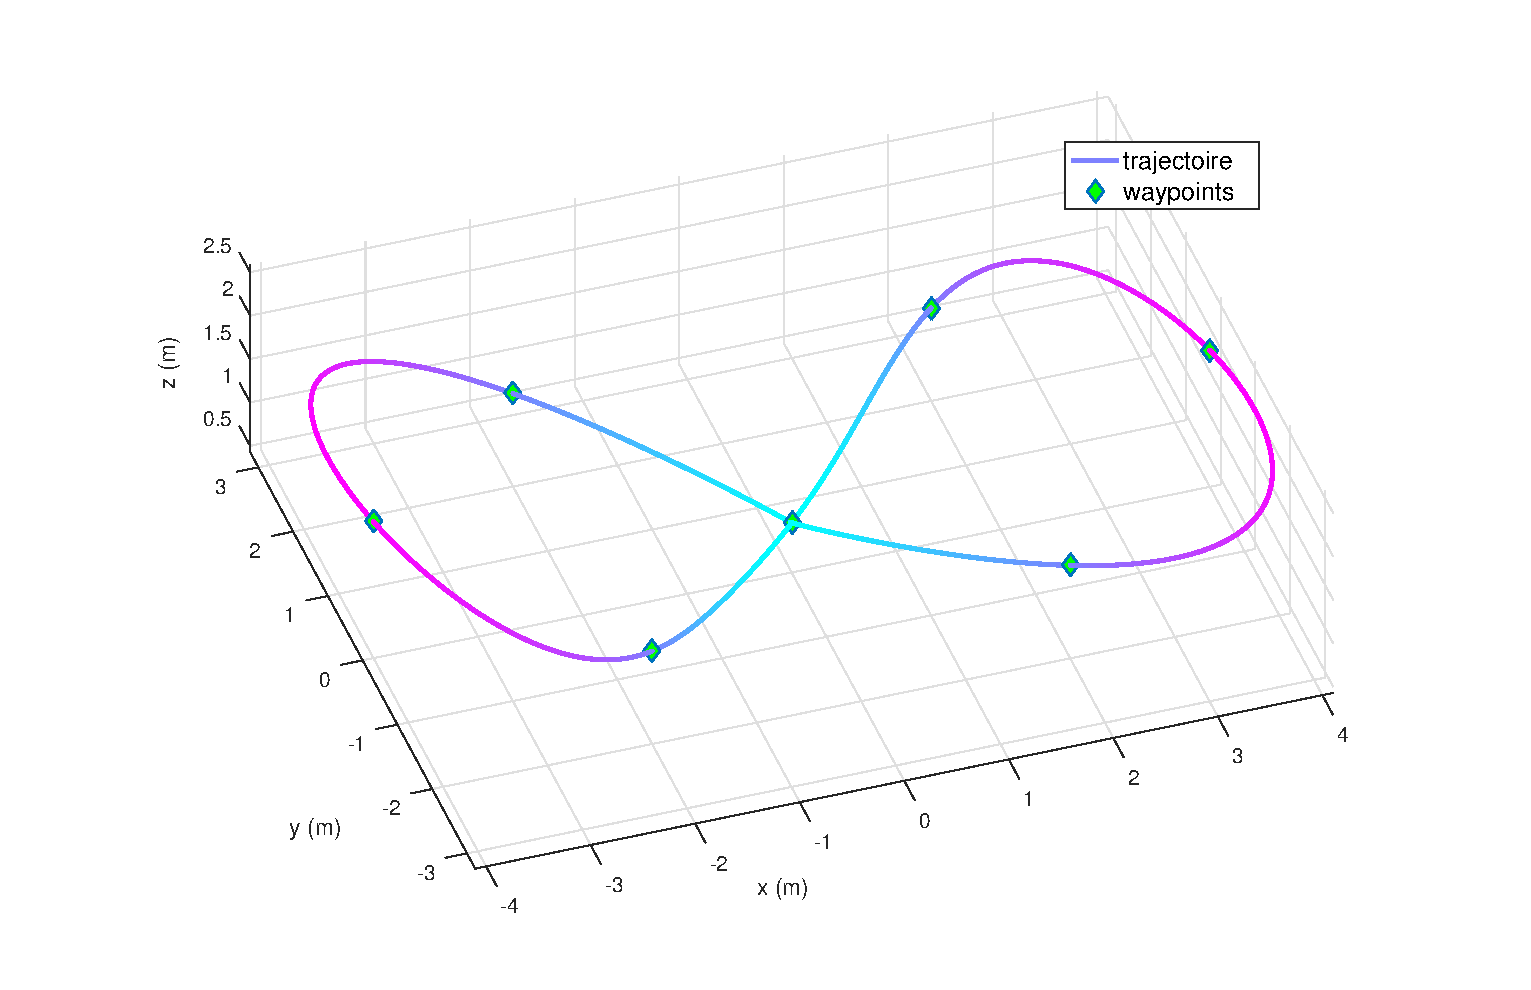
\includegraphics[width=0.9\linewidth]{fig/figure8}
	\caption{Trajectoire en forme de "8"}
	\label{fig:figure8}
\end{figure}

Examinons maintenant la solution du problème QP dans la dimension $x$. En transformant le vecteur $c$ de 54 éléments en une matrice de $n+1 \times m+1$ \textit{i.e.} le nombre de coefficients des polynômes par le nombre de waypoints incluant les conditions initiales. Nous avons la matrice dans l'équation (\ref{eq:solution_figure8}). 

\begin{figure}
\begin{align}\label{eq:solution_figure8}
c = \begin{bmatrix}
  2.3370 &  -8.2665 &   7.9295 &        0 &        0 &        0 &        0  \\
  0.2622 &   0.4434 &   1.6518 &  -4.2073 &  -0.0332 &   4.4075 &   2.0000  \\
  0.1200 &  -0.3732 &  -0.0640 &   1.5901 &  -2.2431 &  -1.0297 &   4.0000  \\
  -0.0206 &   0.0881 &  -0.1308 &   0.0010 &   0.2103 &  -2.1480 &   2.0000 \\
  0.0206 &  -0.0358 &  -0.0000 &  -0.0540 &   0.0000 &  -1.9308 &        0  \\
  -0.1200 &   0.3465 &   0.1308 &   0.0010 &  -0.2103 &  -2.1480 &  -2.0000 \\
  0.2622 &  -1.1297 &   0.0640 &   1.5901 &   2.2431 &  -1.0297 &  -4.0000  \\
  -2.3370 &   5.7554 &  -1.6518 &  -4.2073 &   0.0332 &   4.4075 &  -2.0000 \\
\end{bmatrix}
\end{align}
	\caption{Solution finale en $x$ pour la trajectoire de la figure (\ref{fig:figure8})}
\end{figure}
Donc, chaque ligne représente les coefficients d'un polynôme non-dimensionné dans le temps. Notons que le dernier facteur de chaque polynôme est toujours la valeur d'un des waypoints puisque quand $t=0$ la trajectoire s'évalue au coefficient $c_0$ tel que présenté dans l'équation (\ref{eq:polynomial}). 

Mellinger explique que pour toute solution optimale non-dimentionnée $\tilde{r}^*(\tau)$ où $\tau$ est le temps non-dimensionné, il est possible de faire une mise à l'échelle temporelle et spatiale de la solution. Par exemple Si nous voulons rallonger les temps d'arrivé à chaque waypoint par un facteur $\alpha$ nous pouvons appliquer le changement de variable $t_i = \alpha \tau_i$ ce qui donne lieu à une nouvelle solution
\begin{align*}
	r^*(t) = \tilde{r}^*(t/\alpha)
\end{align*}
Nous pouvons profiter de cette propriété pour satisfaire des contraintes \textit{a posteriori} sur les accélérations demandées au véhicule. Par exemple dans la figure (\ref{fig:comparaison_nondimensionalisation}) nous voyons que la solution initiale nous demande des accélérations de près de $7.5 m/s^2$ en $x$ et presque $13 m/s^2$ en $y$. En faisant une mise à l'échelle de la solution avec $\alpha = 2$, nous doublons le temps alloué à la trajectoire et nous obtenons des accélérations plus raisonables sur le véhicule à un maximum de $2 m/s^2$ en $x$ et $3.15 m/s^2$ en $y$

\begin{figure}[h]
  \centering
  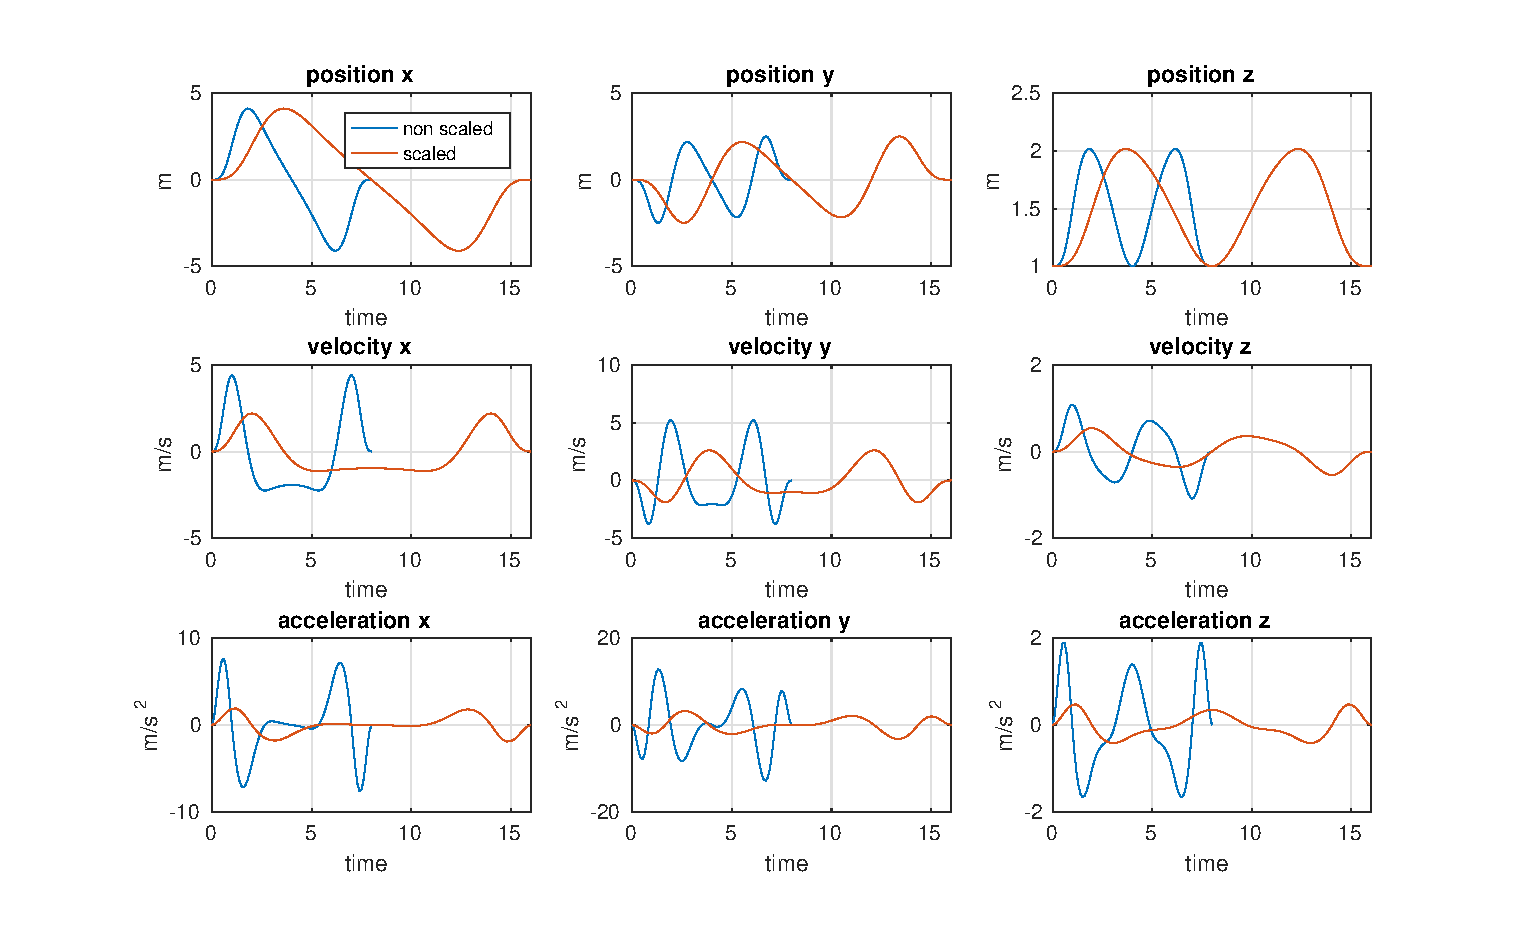
\includegraphics[width=\textwidth ,trim=50 25 65 15, clip]{fig/figure8_derivatives}
  \caption{Comparaison entre la solution non-dimensionnelle et celle mise à l'échelle avec $\alpha = 2$}
  \label{fig:comparaison_nondimensionalisation}
\end{figure}

\subsection{Implémentation finale en C++}
L'intérêt de passer au C++ est d'éventuellement nous permettre d'utiliser le générateur de trajectories sur un vrai véhicule opérant avec le Robot Operating System (ROS) ou du moins, un véhicule simulé avec ROS dans l'environmment de simulation Gazebo. À l'aide de la librairie d'algèbre linéaire Eigen \cite{eigenweb} le transfert de l'essentiel du code a été relativement simple.

\subsubsection{Comparaison de solveurs QP}

Nous avons structuré le code C++ à fin de pouvoir comparer plusieurs solveurs QP dont: OOQP \citep{ooqp}, Gurobi \citep{gurobi}, qpOASES \citep{Ferreau2014} et le \textit{Bound and Linear Equality and Inequality Constraint} (BLEIC) de ALGLIB\cite{alglib}. Nous commençons par reprendre l'exemple de génération d'une trajectoire en "8" avec les mêmes waypoints que ceux de la figure (\ref{fig:figure8}) sans une optimisation sur l'allocation des temps de segment. Pour calculer la valeur finale de la fonction objectif nous faisons une sommation de la valeur de la fonction de coût ($x^T H x$) dans les trois dimensions $x$, $y$ et $z$. Le nombre d'itérations est la somme des itérations requises pour résoudre le problème dans les 3 dimensions. Le temps d'exécution est mesuré à partir du début de l'optimisation et n'inclut pas le temps requis pour bâtir le problème. Pour assurer la cohérence de nos résultats, le temps d'exécution présenté est une moyenne sur 100 essais.

Nous voyons dans le tableau (\ref{table:qp_comparison}) les résultats de nos tests. Nous voyons que OOQP performe beaucoup mieux que les autres solveurs et résout les trois problèmes QP en une seule itération de la même façon que \texttt{quadprog}. Les méthodes simplex de Gurobi prennent plus d'itérations mais sont comparables en termes de temps d'exécution à la méthode barrière par défaut. qpOASES et BLEIC sont les pires en termes de performance, se basant sur la méthode de l'ensemble des contraintes actives. Dans notre problème, cette méthode n'a pas de but puisque toutes nos contraintes sont actives car notre problème ne comporte que des contraintes d'égalitées. Nous remarquons tout de même que tous les solveurs réussissent à se rendre au même minimum, la différence en \texttt{quadprog} et les autres résultats peut se résumer à une erreur d'arrondissement.

\begin{table}[htp]
	\centering
	\begin{tabular}{ |c|c|c|c|c| } 
 \hline
 Solveur & Type & n. itér. [$x$, $y$, $z$] & $f(x)$ & Temps exéc. (ns) \\ 
 \hline
	Matlab \texttt{quadprog} & Primal-Dual point intérieur & [1 1 1] & 59 859.09 & 10 071 990  \\
	OOQP & Primal-Dual point intérieur & [1 1 1] & 59 859.10 & 230 939\\
	Gurobi & Barrière & [10 10 7] & 59 859.10 & 2 786 326\\
	& Primal-Simplex & [7 7 7] & 59 859.10 & 1 940 684\\
	& Dual-Simplex & [65 65 65] & 59 859.10 & 2 375 172\\
	qpOASES & Online active set & [6 6 6] & 59 856.10 & 3 896 080\\
	ALGLIB QP-BLEIC & Active set& [[7 11] [7 10] [8 11]] & 59 856.10 & 93 946 093\\
 \hline
\end{tabular}
	\caption{Comparaison des solveurs QP. L'algorithme QP-BLEIC donne les "outer iterations" et les "inner iterations".}
	\label{table:qp_comparison}
\end{table}

\subsubsection{Comparaison des solveurs non-linéaires}
Pour remplacer \texttt{fmincon} en C++ nous avons eu recours à BLEIC et à la méthode \textit{Sequential Least-Squares Quadratic Programming} NLopt \cite{nlopt}. Malheureusement nous voulions aussi tenter d'autres algorithmes tel que BFGS et le Lagrangien augmenté mais nous n'avons pas réussis à les faire fonctionner. À la lumière des résultats du tableau (\ref{table:qp_comparison}) nous avons utilisé OOQP comme solveur interne pour évaluer $f(x)$.

Dans le tableau (\ref{table:nl_comparison}) nous voyons que l'algorithme BLEIC est plus performant en termes d'itérations que \texttt{fmincon} pour un temps d'exécution deux ordres de grandeurs plus petit. NLopt SLSQP performe beaucoup d'itérations mais avec un temps équivalent à BLEIC. Cependant, la chose la plus important à remarquer ici est le fait que cette optimisation faite par dessus l'optimisation QP permet d'atteindre une valeur de fonction beaucoup plus petite, peu importe l'algorithme utilisé.

\begin{table}[htp]
	\centering
	\begin{tabular}{ |c|c|c|c|c|c| } 
 \hline
 Solveur & Type & n. itér. & $f_0(x)$ & $f(x)$ & Temps exéc. (ms) \\ 
 \hline
	Matlab \texttt{fmincon} & Point intérieur& 17& 59 859.09 & 9 354.66 & 11 965.80\\
	ALGlib BLEIC & Active set & 12 & 59 859.10 & 9 354.70 & 219\\
	NLopt & SLSQP& 59 & 59 859.10 & 9 358.01 & 212\\
%	NLopt & L-BFGS& 59 & 59 859.10 & 9 358.01 & 214\\
%	NLopt & Newton tronqué préconditionné& 59 & 59 859.10 & 9358.01 & 212\\
%	NLopt & Lagrangien Augmenté & 59 & 59 859.10 & 9358.01 & 212\\
	\hline
\end{tabular}
	\caption{Comparaison des solveurs non-linéaires}
	\label{table:nl_comparison}
\end{table}

